% Options for packages loaded elsewhere
\PassOptionsToPackage{unicode}{hyperref}
\PassOptionsToPackage{hyphens}{url}
\PassOptionsToPackage{space}{xeCJK}
%
\documentclass[
  10pt,
  ignorenonframetext,
  aspectratio=169,
  t]{beamer}
\usepackage{pgfpages}
\setbeamertemplate{caption}[numbered]
\setbeamertemplate{caption label separator}{: }
\setbeamercolor{caption name}{fg=normal text.fg}
\beamertemplatenavigationsymbolsempty
% Prevent slide breaks in the middle of a paragraph
\widowpenalties 1 10000
\raggedbottom
\setbeamertemplate{part page}{
  \centering
  \begin{beamercolorbox}[sep=16pt,center]{part title}
    \usebeamerfont{part title}\insertpart\par
  \end{beamercolorbox}
}
\setbeamertemplate{section page}{
  \centering
  \begin{beamercolorbox}[sep=12pt,center]{part title}
    \usebeamerfont{section title}\insertsection\par
  \end{beamercolorbox}
}
\setbeamertemplate{subsection page}{
  \centering
  \begin{beamercolorbox}[sep=8pt,center]{part title}
    \usebeamerfont{subsection title}\insertsubsection\par
  \end{beamercolorbox}
}
\AtBeginPart{
  \frame{\partpage}
}
\AtBeginSection{
  \ifbibliography
  \else
    \frame{\sectionpage}
  \fi
}
\AtBeginSubsection{
  \frame{\subsectionpage}
}
\usepackage{amsmath,amssymb}
\usepackage{iftex}
\ifPDFTeX
  \usepackage[T1]{fontenc}
  \usepackage[utf8]{inputenc}
  \usepackage{textcomp} % provide euro and other symbols
\else % if luatex or xetex
  \usepackage{unicode-math} % this also loads fontspec
  \defaultfontfeatures{Scale=MatchLowercase}
  \defaultfontfeatures[\rmfamily]{Ligatures=TeX,Scale=1}
\fi
\usepackage{lmodern}
\usetheme[]{Madrid}
\usefonttheme{serif} % use mainfont rather than sansfont for slide text
\ifPDFTeX\else
  % xetex/luatex font selection
  \setmainfont[]{DejaVu Sans}
  \setmonofont[]{DejaVu Sans Mono}
  \ifXeTeX
    \usepackage{xeCJK}
    \setCJKmainfont[]{Noto Serif CJK SC}
          \fi
  \ifLuaTeX
    \usepackage[]{luatexja-fontspec}
    \setmainjfont[]{Noto Serif CJK SC}
  \fi
\fi
% Use upquote if available, for straight quotes in verbatim environments
\IfFileExists{upquote.sty}{\usepackage{upquote}}{}
\IfFileExists{microtype.sty}{% use microtype if available
  \usepackage[]{microtype}
  \UseMicrotypeSet[protrusion]{basicmath} % disable protrusion for tt fonts
}{}
\makeatletter
\@ifundefined{KOMAClassName}{% if non-KOMA class
  \IfFileExists{parskip.sty}{%
    \usepackage{parskip}
  }{% else
    \setlength{\parindent}{0pt}
    \setlength{\parskip}{6pt plus 2pt minus 1pt}}
}{% if KOMA class
  \KOMAoptions{parskip=half}}
\makeatother
\usepackage{xcolor}
\newif\ifbibliography
\usepackage{color}
\usepackage{fancyvrb}
\newcommand{\VerbBar}{|}
\newcommand{\VERB}{\Verb[commandchars=\\\{\}]}
\DefineVerbatimEnvironment{Highlighting}{Verbatim}{commandchars=\\\{\}}
% Add ',fontsize=\small' for more characters per line
\newenvironment{Shaded}{}{}
\newcommand{\AlertTok}[1]{\textcolor[rgb]{1.00,0.00,0.00}{\textbf{#1}}}
\newcommand{\AnnotationTok}[1]{\textcolor[rgb]{0.38,0.63,0.69}{\textbf{\textit{#1}}}}
\newcommand{\AttributeTok}[1]{\textcolor[rgb]{0.49,0.56,0.16}{#1}}
\newcommand{\BaseNTok}[1]{\textcolor[rgb]{0.25,0.63,0.44}{#1}}
\newcommand{\BuiltInTok}[1]{\textcolor[rgb]{0.00,0.50,0.00}{#1}}
\newcommand{\CharTok}[1]{\textcolor[rgb]{0.25,0.44,0.63}{#1}}
\newcommand{\CommentTok}[1]{\textcolor[rgb]{0.38,0.63,0.69}{\textit{#1}}}
\newcommand{\CommentVarTok}[1]{\textcolor[rgb]{0.38,0.63,0.69}{\textbf{\textit{#1}}}}
\newcommand{\ConstantTok}[1]{\textcolor[rgb]{0.53,0.00,0.00}{#1}}
\newcommand{\ControlFlowTok}[1]{\textcolor[rgb]{0.00,0.44,0.13}{\textbf{#1}}}
\newcommand{\DataTypeTok}[1]{\textcolor[rgb]{0.56,0.13,0.00}{#1}}
\newcommand{\DecValTok}[1]{\textcolor[rgb]{0.25,0.63,0.44}{#1}}
\newcommand{\DocumentationTok}[1]{\textcolor[rgb]{0.73,0.13,0.13}{\textit{#1}}}
\newcommand{\ErrorTok}[1]{\textcolor[rgb]{1.00,0.00,0.00}{\textbf{#1}}}
\newcommand{\ExtensionTok}[1]{#1}
\newcommand{\FloatTok}[1]{\textcolor[rgb]{0.25,0.63,0.44}{#1}}
\newcommand{\FunctionTok}[1]{\textcolor[rgb]{0.02,0.16,0.49}{#1}}
\newcommand{\ImportTok}[1]{\textcolor[rgb]{0.00,0.50,0.00}{\textbf{#1}}}
\newcommand{\InformationTok}[1]{\textcolor[rgb]{0.38,0.63,0.69}{\textbf{\textit{#1}}}}
\newcommand{\KeywordTok}[1]{\textcolor[rgb]{0.00,0.44,0.13}{\textbf{#1}}}
\newcommand{\NormalTok}[1]{#1}
\newcommand{\OperatorTok}[1]{\textcolor[rgb]{0.40,0.40,0.40}{#1}}
\newcommand{\OtherTok}[1]{\textcolor[rgb]{0.00,0.44,0.13}{#1}}
\newcommand{\PreprocessorTok}[1]{\textcolor[rgb]{0.74,0.48,0.00}{#1}}
\newcommand{\RegionMarkerTok}[1]{#1}
\newcommand{\SpecialCharTok}[1]{\textcolor[rgb]{0.25,0.44,0.63}{#1}}
\newcommand{\SpecialStringTok}[1]{\textcolor[rgb]{0.73,0.40,0.53}{#1}}
\newcommand{\StringTok}[1]{\textcolor[rgb]{0.25,0.44,0.63}{#1}}
\newcommand{\VariableTok}[1]{\textcolor[rgb]{0.10,0.09,0.49}{#1}}
\newcommand{\VerbatimStringTok}[1]{\textcolor[rgb]{0.25,0.44,0.63}{#1}}
\newcommand{\WarningTok}[1]{\textcolor[rgb]{0.38,0.63,0.69}{\textbf{\textit{#1}}}}
\usepackage{longtable,booktabs,array}
\usepackage{calc} % for calculating minipage widths
\usepackage{caption}
% Make caption package work with longtable
\makeatletter
\def\fnum@table{\tablename~\thetable}
\makeatother
\usepackage{graphicx}
\makeatletter
\def\maxwidth{\ifdim\Gin@nat@width>\linewidth\linewidth\else\Gin@nat@width\fi}
\def\maxheight{\ifdim\Gin@nat@height>\textheight\textheight\else\Gin@nat@height\fi}
\makeatother
% Scale images if necessary, so that they will not overflow the page
% margins by default, and it is still possible to overwrite the defaults
% using explicit options in \includegraphics[width, height, ...]{}
\setkeys{Gin}{width=\maxwidth,height=\maxheight,keepaspectratio}
% Set default figure placement to htbp
\makeatletter
\def\fps@figure{htbp}
\makeatother
\setlength{\emergencystretch}{3em} % prevent overfull lines
\providecommand{\tightlist}{%
  \setlength{\itemsep}{0pt}\setlength{\parskip}{0pt}}
\setcounter{secnumdepth}{-\maxdimen} % remove section numbering
% Tighten vertical rhythm so dense slides fit on a single frame.
\usepackage{etoolbox}
\setlength{\parskip}{3pt plus 1pt minus 1pt}
\setbeamertemplate{itemize/enumerate body begin}{\small}
\setbeamertemplate{itemize/enumerate subbody begin}{\footnotesize}
\AtBeginEnvironment{itemize}{\setlength{\itemsep}{2pt}\setlength{\topsep}{2pt}}
\AtBeginEnvironment{enumerate}{\setlength{\itemsep}{2pt}\setlength{\topsep}{2pt}}
% Shrink code listings and tables so long lines do not force a page break.
\AtBeginEnvironment{Highlighting}{\footnotesize}
\AtBeginEnvironment{verbatim}{\footnotesize}
\AtBeginEnvironment{longtable}{\footnotesize}
\ifLuaTeX
  \usepackage{selnolig}  % disable illegal ligatures
\fi
\IfFileExists{bookmark.sty}{\usepackage{bookmark}}{\usepackage{hyperref}}
\IfFileExists{xurl.sty}{\usepackage{xurl}}{} % add URL line breaks if available
\urlstyle{same}
\hypersetup{
  pdftitle={AgentCore as the Sandbox in Agentic RL},
  pdfauthor={Kaige Yang --- Senior Applied Scientist, AWS},
  hidelinks,
  pdfcreator={LaTeX via pandoc}}

\title{AgentCore as the Sandbox in Agentic RL}
\subtitle{Agentic RL · AgentCore · Integrating AgentCore into slime ·
Demos}
\author{Kaige Yang --- Senior Applied Scientist, AWS}
\date{September 25, 2026}

\setbeamertemplate{frametitle continuation}[from second]
\begin{document}
\frame{\titlepage}

\begin{frame}[fragile,allowframebreaks]{Purpose and thesis}
\protect\hypertarget{purpose-and-thesis}{}
A \textbf{hands-on guide for AWS customers doing agentic RL}, grounded
in a working \textbf{slime + AgentCore} project, the \textbf{official
AgentCore docs} {[}D1{]} and \textbf{6 runnable demos}.

\begin{itemize}
\tightlist
\item
  \textbf{What AgentCore can and cannot do} as an RL sandbox.
\item
  \textbf{How to wire it into a trainer} --- one \texttt{generate} hook
  into slime, no fork.
\item
  \textbf{How to run each demo} --- six numbered step scripts, a few
  knobs, measured smoke numbers.
\end{itemize}

\textbf{Thesis.} The loop has two seams: the \textbf{harness} (the agent
loop) and the \textbf{sandbox} (where untrusted output runs and the
reward is computed). We keep the harness \textbf{in-process} and put
\textbf{AgentCore in the sandbox seam}. Policy is always
\textbf{Qwen3-4B} trained by \textbf{slime}; across demos only the
\textbf{sandbox substrate} and the \textbf{task} change.
\end{frame}

\hypertarget{agentic-rl-pipeline-workflow-architecture}{%
\section{1 · Agentic RL --- pipeline, workflow,
architecture}\label{agentic-rl-pipeline-workflow-architecture}}

\begin{frame}[allowframebreaks]{The agentic-RL loop}
\protect\hypertarget{the-agentic-rl-loop}{}
\begin{figure}
\centering
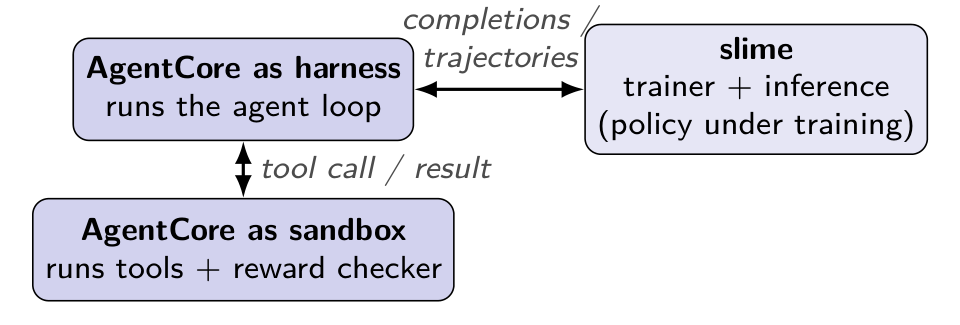
\includegraphics[width=0.78\textwidth,height=\textheight]{figures/fig01_project-theme-two-roles.png}
\caption{AgentCore fills the RL execution roles around a slime trainer.}
\end{figure}

A rollout is a multi-turn \textbf{act → observe → revise} loop: the
policy proposes an action, the \textbf{sandbox} runs it, and a
\textbf{checker} in the sandbox produces the reward. The
\textbf{harness} owns the loop; \textbf{slime} trains on the resulting
samples.
\end{frame}

\begin{frame}[fragile,allowframebreaks]{The harness --- owns the episode}
\protect\hypertarget{the-harness-owns-the-episode}{}
\begin{figure}
\centering
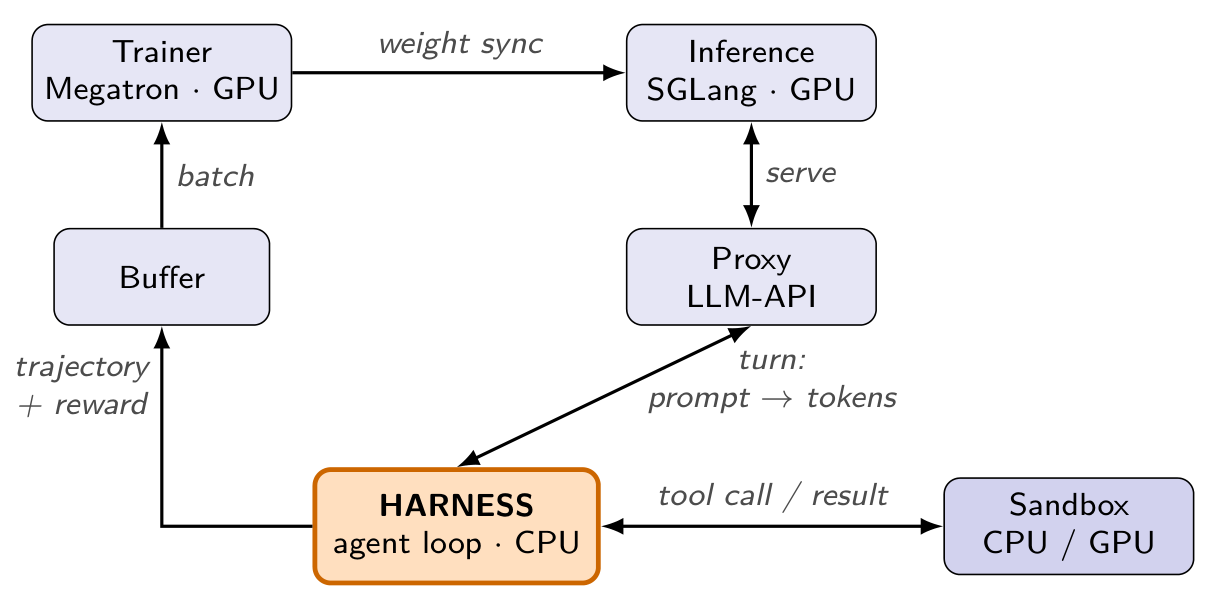
\includegraphics[width=0.42\textwidth,height=\textheight]{figures/fig04_harness-as-hub-dataflow.png}
\caption{The harness as hub --- generation, action, and the record that
becomes training data.}
\end{figure}

\begin{itemize}
\tightlist
\item
  Opens the episode, calls the policy turn by turn, routes actions to
  the sandbox, runs the checker, packs a training \texttt{Sample}.
\item
  The \textbf{only component that sees a whole episode}, so it stamps
  reward, grouping and loss mask.
\item
  A \textbf{proxy} records the \textbf{exact \texttt{token\_ids} +
  logprobs} sampled (\textbf{TITO}); without it training is silently
  off-policy.
\end{itemize}
\end{frame}

\begin{frame}[fragile,allowframebreaks]{slime --- trainer + asynchronous rollout}
\protect\hypertarget{slime-trainer-asynchronous-rollout}{}
\begin{figure}
\centering
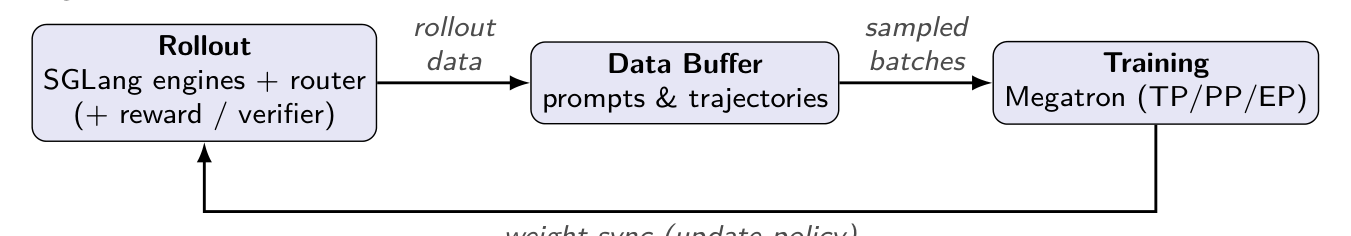
\includegraphics[width=0.66\textwidth,height=\textheight]{figures/fig15_slime-architecture.png}
\caption{slime: rollout generation → data buffer → Megatron training,
decoupled.}
\end{figure}

\textbf{slime} {[}9{]} = \textbf{Megatron} (training) + \textbf{SGLang}
(rollout) behind a router, bridged by a Data Buffer. Agentic workloads
plug in as a \textbf{custom rollout-generation hook}; this is where the
harness and the AgentCore sandbox live. Rollout and training run
\textbf{async} (\texttt{MODE=B}, GRPO).
\end{frame}

\begin{frame}[fragile,allowframebreaks]{Tasks --- seed, run, check, reward}
\protect\hypertarget{tasks-seed-run-check-reward}{}
One \textbf{task-agnostic} harness; a task family changes only
\textbf{prompt + seed files + checker}. All \textbf{RLVR}: binary
1.0/0.0 from a checker, no LLM judge.

\begin{Shaded}
\begin{Highlighting}[]
\ControlFlowTok{for}\NormalTok{ name, content }\KeywordTok{in}\NormalTok{ task.setup\_files():}
    \ControlFlowTok{await}\NormalTok{ sandbox.write\_file(name, content)}
\ControlFlowTok{for}\NormalTok{ \_ }\KeywordTok{in} \BuiltInTok{range}\NormalTok{(task.max\_turns):}
\NormalTok{    text }\OperatorTok{=} \ControlFlowTok{await}\NormalTok{ policy.complete(messages)                 }\CommentTok{\# model turn (via proxy)}
    \ControlFlowTok{await}\NormalTok{ sandbox.write\_file(task.artifact\_filename, task.extract\_submission(text))}
\NormalTok{    exit\_code, out, err }\OperatorTok{=} \ControlFlowTok{await}\NormalTok{ sandbox.}\BuiltInTok{exec}\NormalTok{(}\StringTok{"python3 run\_checks.py"}\NormalTok{, timeout}\OperatorTok{=}\DecValTok{60}\NormalTok{)}
    \ControlFlowTok{if}\NormalTok{ exit\_code }\OperatorTok{==} \DecValTok{0}\NormalTok{: solved }\OperatorTok{=} \VariableTok{True}\OperatorTok{;} \ControlFlowTok{break}
\NormalTok{    messages.append(task.observation(exit\_code, out, err)) }\CommentTok{\# feed failure back}
\NormalTok{reward }\OperatorTok{=}\NormalTok{ task.reward(}\DecValTok{0} \ControlFlowTok{if}\NormalTok{ solved }\ControlFlowTok{else} \DecValTok{1}\NormalTok{)}
\end{Highlighting}
\end{Shaded}

\textbf{The checker runs inside the sandbox --- the sandbox is the
reward source.} Frontier labs (DeepSeek-R1 {[}2{]}, Qwen3 {[}3{]}, Kimi
K2 {[}5{]}) train the same way against executable verifiers.
\end{frame}

\begin{frame}[fragile,allowframebreaks]{Scaling --- throughput = min(inference, sandbox,
harness)}
\protect\hypertarget{scaling-throughput-mininference-sandbox-harness}{}
\begin{figure}
\centering
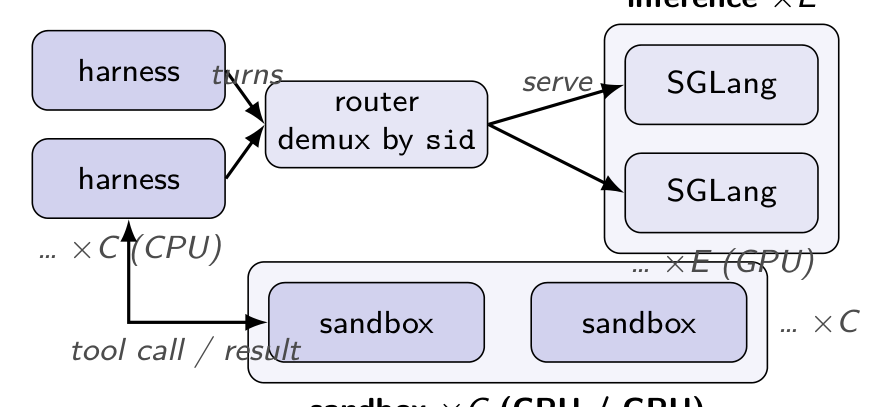
\includegraphics[width=0.46\textwidth,height=\textheight]{figures/fig08_scaled-rollout-C-E-C.png}
\caption{Scaled rollout --- C harnesses and sandboxes feeding E
inference engines.}
\end{figure}

Scale two tiers and the bottleneck moves, so \textbf{diagnose first}
with \texttt{perf/sglang\_gen\_ms\_*} vs \texttt{perf/sandbox\_ms\_*}:

\begin{itemize}
\tightlist
\item
  \textbf{Generation dominates} → inference-bound: add SGLang replicas
  (e.g.~long-reasoning math).
\item
  \textbf{Sandbox dominates} → sandbox-bound: add sandbox concurrency or
  instances (e.g.~KernelBench \texttt{nvcc}).
\end{itemize}
\end{frame}

\hypertarget{agentcore-foundation-concepts-and-workflow}{%
\section{2 · AgentCore --- foundation concepts and
workflow}\label{agentcore-foundation-concepts-and-workflow}}

\begin{frame}[fragile,allowframebreaks]{AgentCore basics --- can / cannot}
\protect\hypertarget{agentcore-basics-can-cannot}{}
\begin{figure}
\centering
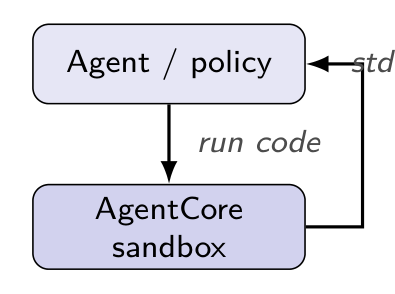
\includegraphics[width=0.3\textwidth,height=\textheight]{figures/fig16_agentcore-two-roles.png}
\caption{AgentCore's two RL roles --- host the harness and/or be the
sandbox.}
\end{figure}

\begin{itemize}
\tightlist
\item
  \textbf{Runtime} --- serverless, \textbf{per-session isolated
  compute}, invoked with \texttt{InvokeAgentRuntime} (SigV4) {[}D2,
  D8{]}.
\item
  \textbf{Code Interpreter} --- managed CPU sandbox, Python/JS/TS
  {[}D6{]}. Also Browser, Gateway, Memory, Identity, Observability
  {[}D13{]}.
\item
  \textbf{Cannot:} GPU on a microVM (GPU is on \textbf{Instances} only)
  {[}D5{]}; cross-session GPU time-slicing; microVM sessions past 8 h
  {[}D3{]}.
\end{itemize}
\end{frame}

\begin{frame}[fragile,allowframebreaks]{Two compute substrates}
\protect\hypertarget{two-compute-substrates}{}
\begin{longtable}[]{@{}
  >{\raggedright\arraybackslash}p{(\columnwidth - 4\tabcolsep) * \real{0.3333}}
  >{\raggedright\arraybackslash}p{(\columnwidth - 4\tabcolsep) * \real{0.3333}}
  >{\raggedright\arraybackslash}p{(\columnwidth - 4\tabcolsep) * \real{0.3333}}@{}}
\toprule\noalign{}
\begin{minipage}[b]{\linewidth}\raggedright
\end{minipage} & \begin{minipage}[b]{\linewidth}\raggedright
\textbf{microVM} (serverless, CPU)
\end{minipage} & \begin{minipage}[b]{\linewidth}\raggedright
\textbf{Instances} (EC2 via a capacity provider)
\end{minipage} \\
\midrule\noalign{}
\endhead
Compute & own guest kernel, \textbf{CPU only} & \texttt{m5} (CPU) ·
\texttt{g6} / \texttt{g5} \ldots{} (\textbf{GPU}) \\
Arch / image cap & \textbf{arm64}, \textasciitilde{}\textbf{2 GB} &
\textbf{amd64}, instance root disk \\
Cold start & \textasciitilde1--2 s & \textasciitilde60--80 s (EC2
launch) \\
Session length & up to 8 h (15-min idle) & up to 14 days \\
Our reuse policy & fresh microVM per episode & \textbf{warm-shared}
instance, fresh env per episode \\
Loop code & identical & identical --- only the Runtime ARN differs \\
\bottomrule\noalign{}
\end{longtable}
\end{frame}

\begin{frame}[fragile,allowframebreaks]{Runtime / session / compute --- 1 : N : 1}
\protect\hypertarget{runtime-session-compute-1-n-1}{}
\begin{figure}
\centering
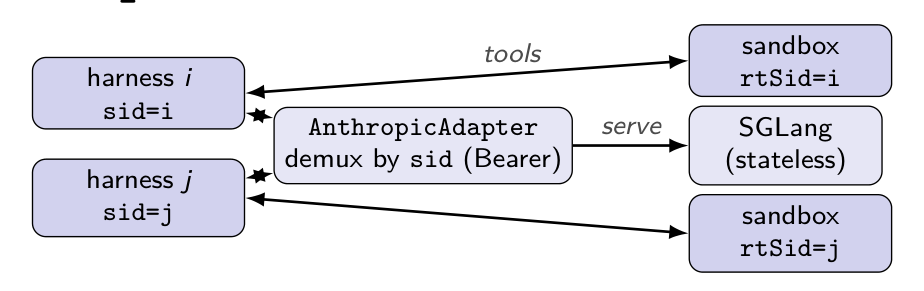
\includegraphics[width=0.6\textwidth,height=\textheight]{figures/fig34_session-id-routing.png}
\caption{Everything keyed by \texttt{runtimeSessionId} --- one isolated
compute unit per session.}
\end{figure}

\begin{itemize}
\tightlist
\item
  \textbf{Runtime} = a stateless template: one image, one ARN.
\item
  \textbf{Session} = one \texttt{runtimeSessionId} (≥33 chars). The
  first invoke under a new id \textbf{cold-starts} its own microVM or
  instance; the same id routes back to it.
\item
  One Runtime serves many sessions; each session maps to exactly one
  compute unit. \textbf{Runtimes track images, not tasks.}
\end{itemize}
\end{frame}

\begin{frame}[fragile,allowframebreaks]{Lifecycle and latency}
\protect\hypertarget{lifecycle-and-latency}{}
\begin{itemize}
\tightlist
\item
  \textbf{Launch:} no ``create session'' API. The first
  \texttt{InvokeAgentRuntime} under a new id provisions compute
  {[}D2{]}.
\item
  \textbf{Terminate:} idle timeout (15 min, resets per invoke), max
  lifetime (microVM 8 h, Instances 14 d), or \texttt{StopRuntimeSession}
  {[}D3, D4, D12{]}; memory is sanitized.
\item
  \textbf{Latency:} no published cold-start number, so \textbf{measure
  it}. Every sandbox op logs \texttt{{[}sbx-op{]}} and every generation
  \texttt{{[}sglang-gen{]}} → \texttt{perf/sandbox\_ms\_*},
  \texttt{perf/sandbox\_open\_*} (cold vs warm),
  \texttt{perf/sglang\_gen\_ms\_*}.
\end{itemize}
\end{frame}

\begin{frame}[fragile,allowframebreaks]{Build and deploy a Runtime}
\protect\hypertarget{build-and-deploy-a-runtime}{}
\begin{enumerate}
\tightlist
\item
  Build the sandbox image (\texttt{docker\ buildx}: \textbf{arm64} for
  microVM, \textbf{amd64} for Instances) and push to ECR.
\item
  \texttt{CreateAgentRuntime} with \texttt{containerConfiguration}
  {[}D9{]}. The image serves a \texttt{BedrockAgentCoreApp}
  (\texttt{sandbox\_server\_agent.py}) with ops \texttt{write\_file} /
  \texttt{exec} / \texttt{read\_file}.
\item
  For Instances: \texttt{CreateCapacityProvider} (\texttt{m5} or
  \texttt{g6.xlarge}, VPC subnets/SGs, idle timeout) and attach it
  {[}D5{]}.
\item
  IAM: an execution role (ECR pull, logs) plus an operator role that can
  \texttt{InvokeAgentRuntime}.
\end{enumerate}

Every demo wraps these as \texttt{2\_build\_image.sh} →
\texttt{3\_push\_ecr.sh} → \texttt{4\_deploy\_runtime.sh} (§4).
\end{frame}

\begin{frame}[fragile,allowframebreaks]{The GPU limit --- one whole GPU per session}
\protect\hypertarget{the-gpu-limit-one-whole-gpu-per-session}{}
\begin{itemize}
\tightlist
\item
  1 \texttt{runtimeSessionId} = 1 EC2 instance = \textbf{whole GPU(s)};
  no documented cross-session sharing; \textbf{no MIG on L4} {[}D5{]}.
\item
  \textbf{Isolated scaling} = more instances (N× cost). \textbf{Shared
  GPU} = many episodes inside one session, which must be mutually
  trusted.
\item
  Our pattern: a \textbf{Ray farm inside one session}
  (\texttt{num\_gpus=0.5} actors, a per-process memory cap, an
  \texttt{nvcc} lock).
\end{itemize}
\end{frame}

\hypertarget{integrating-agentcore-into-slime}{%
\section{3 · Integrating AgentCore into
slime}\label{integrating-agentcore-into-slime}}

\begin{frame}[fragile,allowframebreaks]{Two hooks, no fork}
\protect\hypertarget{two-hooks-no-fork}{}
\begin{figure}
\centering
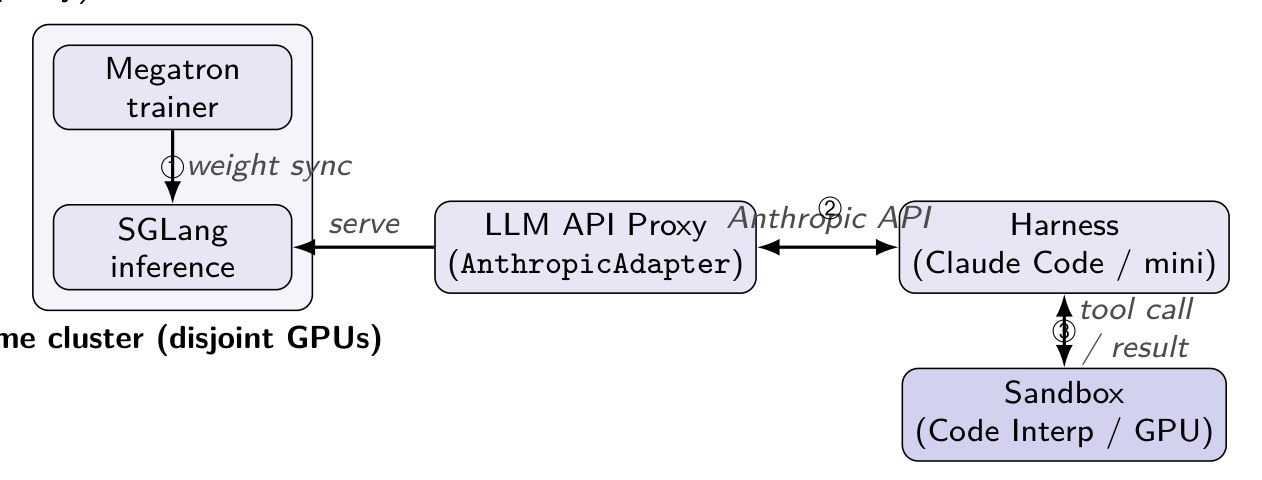
\includegraphics[width=0.64\textwidth,height=\textheight]{figures/fig19_three-decoupling-seams.png}
\caption{The three decoupling seams --- harness, inference, sandbox.}
\end{figure}

\begin{itemize}
\tightlist
\item
  \texttt{-\/-custom-generate-function-path} →
  \texttt{generate.generate} (runs the harness, records turns).
\item
  \texttt{-\/-custom-rm-path} → the reward.
\item
  Each sandbox op is one
  \texttt{invoke\_agent\_runtime(ARN,\ session\_id)}, offloaded with
  \texttt{asyncio.to\_thread}, so \textbf{N episodes run concurrently}.
\end{itemize}
\end{frame}

\begin{frame}[fragile,allowframebreaks]{The call path}
\protect\hypertarget{the-call-path}{}
\begin{figure}
\centering
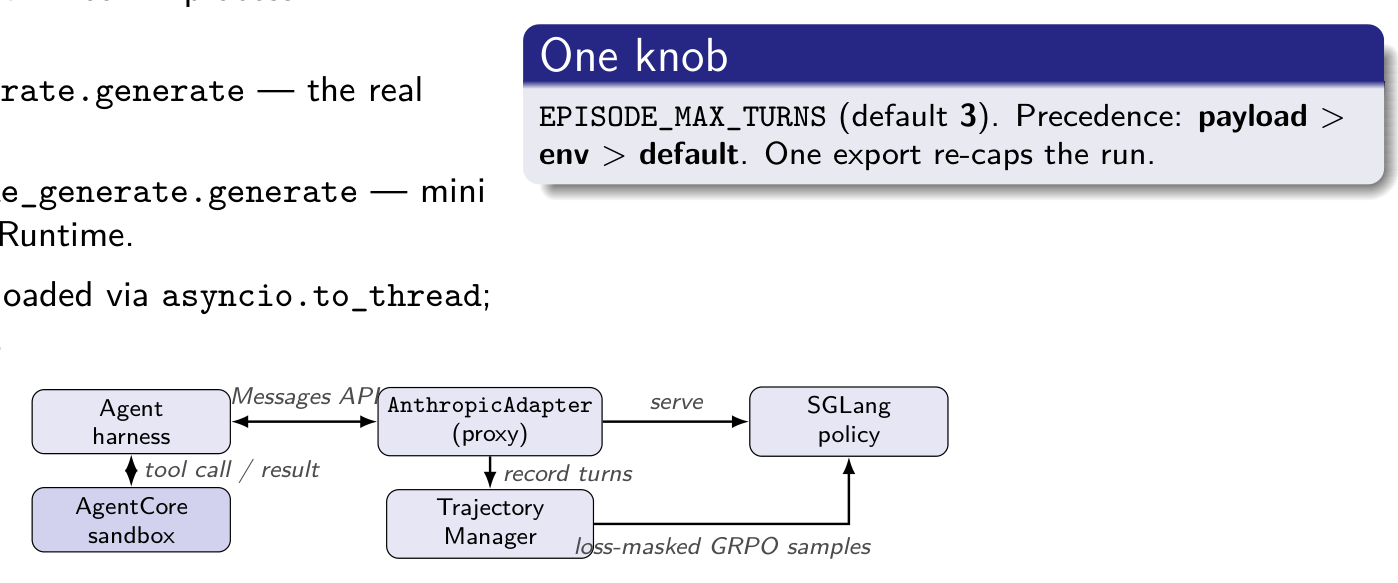
\includegraphics[width=0.5\textwidth,height=\textheight]{figures/fig21_generate-hook.png}
\caption{The generate hook --- harness → proxy → policy, producing a
loss-masked trajectory.}
\end{figure}

\begin{Shaded}
\begin{Highlighting}[]
\ControlFlowTok{async} \KeywordTok{def}\NormalTok{ generate(args, sample, sampling\_params):        }\CommentTok{\# slime hook}
\NormalTok{    task }\OperatorTok{=}\NormalTok{ task\_from\_dict(sample.metadata[}\StringTok{"task"}\NormalTok{])}
    \ControlFlowTok{async} \ControlFlowTok{with}\NormalTok{ make\_sandbox(os.environ[}\StringTok{"SANDBOX"}\NormalTok{]) }\ImportTok{as}\NormalTok{ sb:  }\CommentTok{\# session opened / closed here}
\NormalTok{        traj }\OperatorTok{=} \ControlFlowTok{await}\NormalTok{ run\_episode(task, policy, sb)}
    \ControlFlowTok{return}\NormalTok{ build\_token\_stream(traj, sample)               }\CommentTok{\# loss{-}masked Sample}
\end{Highlighting}
\end{Shaded}

\texttt{\_\_aexit\_\_} ends the session the moment the episode returns
--- one teardown path for every demo.
\end{frame}

\begin{frame}[fragile,allowframebreaks]{Sandbox backends and ARN wiring}
\protect\hypertarget{sandbox-backends-and-arn-wiring}{}
\textbf{ARN wiring} (step 4 → \texttt{deploy/runtime.env}):
\texttt{AGENTCORE\_SANDBOX\_RUNTIME\_ARN} · \texttt{…\_ARNS}
(round-robin) · \texttt{…\_ARN\_BY\_IMAGE} (JSON).

\small

\begin{longtable}[]{@{}
  >{\raggedright\arraybackslash}p{(\columnwidth - 4\tabcolsep) * \real{0.3333}}
  >{\raggedright\arraybackslash}p{(\columnwidth - 4\tabcolsep) * \real{0.3333}}
  >{\raggedright\arraybackslash}p{(\columnwidth - 4\tabcolsep) * \real{0.3333}}@{}}
\toprule\noalign{}
\begin{minipage}[b]{\linewidth}\raggedright
\texttt{SANDBOX=}
\end{minipage} & \begin{minipage}[b]{\linewidth}\raggedright
Substrate
\end{minipage} & \begin{minipage}[b]{\linewidth}\raggedright
Used by
\end{minipage} \\
\midrule\noalign{}
\endhead
\texttt{agentcore} & managed Code Interpreter microVM & offline
comparisons \\
\texttt{agentcore-runtime} & custom Runtime, one session per episode &
CPU demos \\
\texttt{agentcore-ray-farm} & one shared \texttt{runtimeSessionId} + a
per-episode \texttt{sub\_session} & \texttt{demo\_gpu\_single},
\texttt{VARIANT=bigimage} \\
local farm (\texttt{:8080}) & same contract on local GPUs 6,7 &
\texttt{demo\_gpu\_farm}, \texttt{LOCAL\_GPU=1} \\
\bottomrule\noalign{}
\end{longtable}
\end{frame}

\begin{frame}[fragile,allowframebreaks]{Warm reuse on Instances}
\protect\hypertarget{warm-reuse-on-instances}{}
The Instances substrate cold-boots in \textasciitilde60--80 s, so a
fresh instance per episode lets boot time dominate. Instead:

\begin{itemize}
\tightlist
\item
  \textbf{All episodes share one \texttt{runtimeSessionId}} → one warm
  instance, cold boot paid \textbf{once per run}.
\item
  \textbf{Each episode gets a \texttt{sub\_session}} with a fresh
  isolated working dir (CPU isolates caches too; GPU keeps the CUDA
  kernel cache warm).
\item
  microVMs boot in \textasciitilde1--2 s, so they are \textbf{not}
  reused: one fresh microVM per episode.
\end{itemize}

\textbf{Measured (m5, \texttt{VARIANT=bigimage}):} cold boots
\textbf{201 → 1}; 1626 warm ops at \textasciitilde120--350 ms vs
\textasciitilde65--73 s cold.
\end{frame}

\begin{frame}[fragile,allowframebreaks]{Networking --- pull, don't expose}
\protect\hypertarget{networking-pull-dont-expose}{}
\begin{figure}
\centering
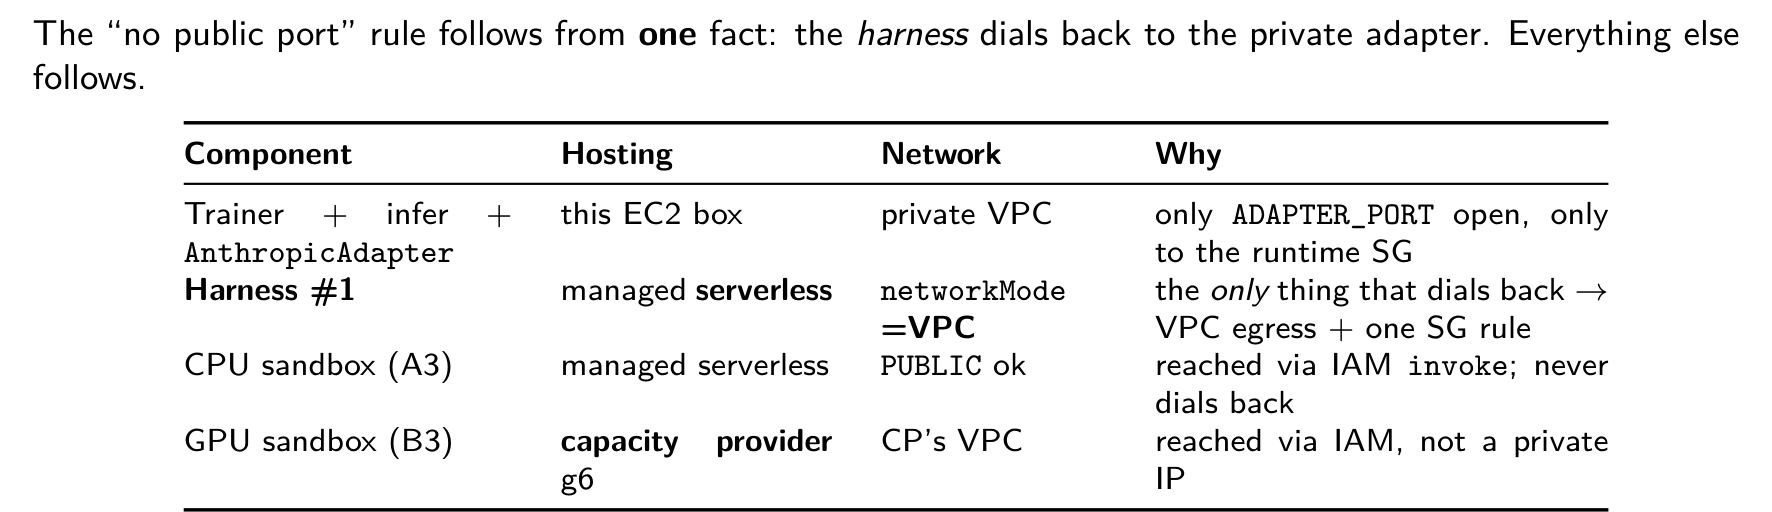
\includegraphics[width=0.62\textwidth,height=\textheight]{figures/fig32_network-posture-per-component.png}
\caption{Network posture per component.}
\end{figure}

Every Runtime is reached by a SigV4 \texttt{invoke\_agent\_runtime},
with \textbf{no inbound port}. Only dial-back (sandbox → harness,
\texttt{demo\_cpu\_branching}) needs ingress: one rule,
tcp/\texttt{ADAPTER\_PORT}, source = the runtime SG, under
\texttt{networkMode=VPC} {[}D10{]}. That requires interface endpoints
(\texttt{ecr.api}, \texttt{ecr.dkr}, \texttt{s3}, \texttt{logs},
\texttt{sts}, \texttt{bedrock-agentcore}) {[}D11{]}; a missing one fails
create with a \textbf{null reason}.
\end{frame}

\hypertarget{demos}{%
\section{4 · Demos}\label{demos}}

\begin{frame}[fragile,allowframebreaks]{Demo catalogue --- 6 demos}
\protect\hypertarget{demo-catalogue-6-demos}{}
\textbf{3 CPU + 2 GPU + 1 experimental.} Run any demo with
\texttt{cd\ code/demos/\textless{}demo\textgreater{}} then
\texttt{1\_prepare\_data.sh} \ldots{} \texttt{6\_cleanup.sh} on the
host. Numbers are 10-step smokes, not convergence.

\scriptsize

\begin{longtable}[]{@{}
  >{\raggedright\arraybackslash}p{(\columnwidth - 4\tabcolsep) * \real{0.2941}}
  >{\raggedright\arraybackslash}p{(\columnwidth - 4\tabcolsep) * \real{0.2059}}
  >{\raggedright\arraybackslash}p{(\columnwidth - 4\tabcolsep) * \real{0.5000}}@{}}
\toprule\noalign{}
\begin{minipage}[b]{\linewidth}\raggedright
Demo
\end{minipage} & \begin{minipage}[b]{\linewidth}\raggedright
Substrate
\end{minipage} & \begin{minipage}[b]{\linewidth}\raggedright
Use case
\end{minipage} \\
\midrule\noalign{}
\endhead
\texttt{demo\_cpu\_tasks} & microVM (\texttt{bigimage}: m5) &
\textbf{Reference:} RLVR on \textasciitilde19 datasets or a mix \\
\texttt{demo\_cpu\_terminalbench} & microVM, \textasciitilde229 images &
one Runtime per task, fresh VM, pre-opened \\
\texttt{demo\_cpu\_scale\_lanes} & 4 microVMs & 4 harness : 4 engines :
4 VMs, 1:1:1 \\
\texttt{demo\_gpu\_single} & \texttt{g6} Instance & KernelBench on one
warm g6 (+ snapshot) \\
\texttt{demo\_gpu\_farm} & local Ray farm & GPU sharing:
\texttt{FARM=fractional} or \texttt{whole} \\
\emph{\texttt{demo\_cpu\_branching}} & microVM + CLI &
\textbf{experimental, blocked:} fan-out \\
\bottomrule\noalign{}
\end{longtable}

\texttt{demo\_cpu\_tasks} also covers \texttt{VARIANT=imagepool} (3
images), \texttt{compare\_backends.py} (custom vs managed Runtime);
\texttt{HEARTBEAT=1} works in every demo (all merged 2026-09-25).
\end{frame}

\begin{frame}[fragile,allowframebreaks]{\texttt{demo\_cpu\_tasks} --- the reference}
\protect\hypertarget{demo_cpu_tasks-the-reference}{}
\textbf{Use case.} RLVR on any dataset through one selector: real HF
\texttt{mbpp} (default) \texttt{gsm8k} \texttt{math500}
\texttt{deepscaler} \texttt{humaneval} \texttt{gretelsql}
\texttt{hotpotqa} \texttt{xlam} \texttt{mcp}, the synthetic family zoo
(\texttt{math} \texttt{sql} \texttt{ctf} \texttt{rag} \ldots), a comma
list, or \texttt{mixed}.

\textbf{Knobs.} \texttt{DATASET=} ·
\texttt{VARIANT=bigimage\textbar{}imagepool} · \texttt{HEARTBEAT=1} ·
\texttt{NR} / \texttt{RB} / \texttt{NS} · \texttt{K} (Runtimes
round-robin) · \texttt{CONC}.

\begin{Shaded}
\begin{Highlighting}[]
\FunctionTok{bash}\NormalTok{ 1\_prepare\_data.sh }\KeywordTok{\&\&} \FunctionTok{bash}\NormalTok{ 2\_build\_image.sh }\KeywordTok{\&\&} \FunctionTok{bash}\NormalTok{ 3\_push\_ecr.sh }\KeywordTok{\&\&} \FunctionTok{bash}\NormalTok{ 4\_deploy\_runtime.sh}
\VariableTok{DATASET}\OperatorTok{=}\NormalTok{gsm8k }\FunctionTok{bash}\NormalTok{ 5\_run.sh        }\CommentTok{\# or DATASET=gsm8k,gretelsql,hotpotqa / DATASET=mixed}
\FunctionTok{bash}\NormalTok{ 6\_cleanup.sh}
\end{Highlighting}
\end{Shaded}

\textbf{Metrics (held-out eval).} \texttt{mbpp} \textbf{trained}
(convergence curve + ablation), smoke 0.69 · \texttt{math} 1.00 ·
\texttt{gsm8k} 0.90 · \texttt{math500} 0.89 · \texttt{deepscaler} 0.78 ·
\texttt{humaneval} 0.85 · \texttt{gretelsql} 0.60 · \texttt{hotpotqa}
0.65 · \texttt{xlam} 1.00 · \texttt{mcp} 1.00 · \texttt{mixed} 0.67.
\end{frame}

\begin{frame}[fragile,allowframebreaks]{\texttt{demo\_cpu\_tasks}
\texttt{VARIANT=bigimage} --- side note}
\protect\hypertarget{demo_cpu_tasks-variantbigimage-side-note}{}
\textbf{Use case.} A \textasciitilde4 GB sandbox image, over the 2 GB
microVM cap, on a warm \textbf{m5} CPU capacity-provider Instance
(amd64). Same trainer, warm-shared session, fresh env per episode.

\begin{Shaded}
\begin{Highlighting}[]
\VariableTok{VARIANT}\OperatorTok{=}\NormalTok{bigimage }\FunctionTok{bash}\NormalTok{ 2\_build\_image.sh }\KeywordTok{\&\&} \VariableTok{VARIANT}\OperatorTok{=}\NormalTok{bigimage }\FunctionTok{bash}\NormalTok{ 3\_push\_ecr.sh}
\VariableTok{VARIANT}\OperatorTok{=}\NormalTok{bigimage }\FunctionTok{bash}\NormalTok{ 4\_deploy\_runtime.sh   }\CommentTok{\# {-}\textgreater{} deploy/runtime.bigimage.env}
\VariableTok{VARIANT}\OperatorTok{=}\NormalTok{bigimage }\FunctionTok{bash}\NormalTok{ 5\_run.sh}
\VariableTok{VARIANT}\OperatorTok{=}\NormalTok{bigimage }\VariableTok{DELETE\_CP}\OperatorTok{=}\NormalTok{1 }\FunctionTok{bash}\NormalTok{ 6\_cleanup.sh}
\end{Highlighting}
\end{Shaded}

\textbf{Metrics.} Trained on m5, \texttt{eval} \textbf{0.76}. Cold boots
\textbf{201 → 1} (8 first-wave opens share one boot within 7.9 s; 215
\texttt{open}/\texttt{close} pairs, each wiping its own dir).
\end{frame}

\begin{frame}[fragile,allowframebreaks]{\texttt{demo\_cpu\_tasks}
\texttt{VARIANT=imagepool} --- a pool of images}
\protect\hypertarget{demo_cpu_tasks-variantimagepool-a-pool-of-images}{}
\textbf{Use case.} Mixed-task RL where families need different software:
a pool of 3 custom images (pandas / scipy / sklearn), one Runtime each,
and each episode routed to its family's image. (Was
\texttt{demo\_cpu\_imagepool}.)

\textbf{Knobs.} \texttt{AGENTCORE\_SANDBOX\_RUNTIME\_ARN\_BY\_IMAGE}
(JSON image → ARN, written by step 4) · \texttt{IMAGES=} (which images
to build) · \texttt{DATASET=imagepool} (set by the variant).

\begin{Shaded}
\begin{Highlighting}[]
\BuiltInTok{cd}\NormalTok{ code/demos/demo\_cpu\_tasks}
\BuiltInTok{export} \VariableTok{VARIANT}\OperatorTok{=}\NormalTok{imagepool}
\FunctionTok{bash}\NormalTok{ 1\_prepare\_data.sh }\KeywordTok{\&\&} \FunctionTok{bash}\NormalTok{ 2\_build\_image.sh    }\CommentTok{\# 3 arm64 images}
\FunctionTok{bash}\NormalTok{ 3\_push\_ecr.sh }\KeywordTok{\&\&} \FunctionTok{bash}\NormalTok{ 4\_deploy\_runtime.sh     }\CommentTok{\# {-}\textgreater{} ARN\_BY\_IMAGE map}
\FunctionTok{bash}\NormalTok{ 5\_run.sh }\KeywordTok{\&\&} \FunctionTok{bash}\NormalTok{ 6\_cleanup.sh}
\end{Highlighting}
\end{Shaded}

\textbf{Metrics.} Smoke (as \texttt{demo\_cpu\_imagepool}) held-out eval
\textbf{1.0} (now \texttt{eval/imagepool}); all 3 images routed from one
batch.
\end{frame}

\begin{frame}[fragile,allowframebreaks]{\texttt{demo\_cpu\_terminalbench}}
\protect\hypertarget{demo_cpu_terminalbench}{}
\textbf{Use case.} Terminal/SWE agents on \textbf{Terminal-Bench}: one
image + Runtime per task (\textasciitilde229), a \textbf{brand-new
microVM per episode} (tasks change the whole OS), and a look-ahead data
source that \textbf{pre-opens} the next 2 batches' sessions to hide the
cold start.

\textbf{Knobs.} \texttt{TB\_PREOPEN\_BATCHES} (default 2 → 64 sessions
booted ahead) · \texttt{HARNESS\_WORKERS} · \texttt{TB\_EXEC\_TIMEOUT}.

\begin{Shaded}
\begin{Highlighting}[]
\FunctionTok{bash}\NormalTok{ 1\_prepare\_data.sh            }\CommentTok{\# fetch Terminal{-}Bench tasks}
\FunctionTok{bash}\NormalTok{ 2\_build\_image.sh             }\CommentTok{\# one image per task (also pushes)}
\FunctionTok{bash}\NormalTok{ 4\_deploy\_runtime.sh          }\CommentTok{\# one Runtime per task {-}\textgreater{} tasks/arn\_by\_image.json}
\FunctionTok{bash}\NormalTok{ 5\_run.sh }\KeywordTok{\&\&} \FunctionTok{bash}\NormalTok{ 6\_cleanup.sh}
\end{Highlighting}
\end{Shaded}

\textbf{Metrics.} 218/229 Runtimes deployed, 166 usable after the oracle
check. First smoke (2026-09-23) passed to ckpt 10: boot fully hidden
(\texttt{open\_wait\_ms} p95 0), but \textasciitilde95 \% of pre-opened
microVM time idle and reward sparse (4/382 solves, eval 0.0). Key
signals: \texttt{{[}demo{]}\ open\_wait\_ms},
\texttt{preopen\_idle\_ms}.
\end{frame}

\begin{frame}[fragile,allowframebreaks]{\texttt{demo\_cpu\_tasks} --- custom Runtime and
\texttt{HEARTBEAT=1}}
\protect\hypertarget{demo_cpu_tasks-custom-runtime-and-heartbeat1}{}
\textbf{Custom vs managed Runtime.}
\texttt{python3\ compare\_backends.py} runs the same episode against the
managed Code Interpreter and \textbf{your own} CPU Runtime: same reward,
only operations differ. Real RL on your Runtime is just
\texttt{AGENTCORE\_SANDBOX\_RUNTIME\_ARNS=\textless{}yours\textgreater{}\ DATASET=deepscaler\ bash\ 5\_run.sh}.
Smoke (as \texttt{demo\_cpu\_customruntime}) \texttt{eval/deepscaler}
\textbf{0.69}.

\textbf{Heartbeat, \texttt{HEARTBEAT=1} (any demo).} During the
weight-sync barrier no ops reach the sandbox, and the 15-min idle
timeout can kill it. A \texttt{SessionKeeper} heartbeat, outside the
harness, keeps the session warm. Knobs: \texttt{HEARTBEAT\_IDLE} (600 s)
· \texttt{HEARTBEAT\_PING\_FRACTION} (0.5).

\begin{Shaded}
\begin{Highlighting}[]
\BuiltInTok{cd}\NormalTok{ code/demos/demo\_cpu\_tasks}
\ExtensionTok{python3}\NormalTok{ compare\_backends.py    }\CommentTok{\# managed vs custom, same reward}
\ExtensionTok{python3}\NormalTok{ heartbeat\_demo.py      }\CommentTok{\# offline, seconds}
\VariableTok{DATASET}\OperatorTok{=}\NormalTok{deepscaler }\VariableTok{HEARTBEAT}\OperatorTok{=}\NormalTok{1 }\FunctionTok{bash}\NormalTok{ 5\_run.sh}
\end{Highlighting}
\end{Shaded}

Smoke (as \texttt{demo\_cpu\_heartbeat}) \texttt{eval/deepscaler}
\textbf{0.71} with the keeper live; the offline probe shows the recovery
arc.
\end{frame}

\begin{frame}[fragile,allowframebreaks]{\texttt{demo\_cpu\_scale\_lanes}}
\protect\hypertarget{demo_cpu_scale_lanes}{}
\textbf{Use case.} Makes
\texttt{throughput\ =\ min(inference,\ sandbox,\ harness)} concrete:
\textbf{4 × 4 × 4 lanes} --- 4 harness workers : 4 TP1 SGLang engines :
4 persistent microVMs, pinned 1:1:1. DeepScaleR, fixed.

\textbf{Knobs.} \texttt{LANES} (4) · \texttt{HARNESS\_WORKERS} ·
\texttt{GPUS\_PER\_ENGINE} (1) · \texttt{LANE\_SANDBOX} (1).

\begin{Shaded}
\begin{Highlighting}[]
\ExtensionTok{python3}\NormalTok{ harness\_scaling\_demo.py   }\CommentTok{\# offline throughput sweep}
\FunctionTok{bash}\NormalTok{ 1\_prepare\_data.sh }\KeywordTok{\&\&} \FunctionTok{bash}\NormalTok{ 2\_build\_image.sh }\KeywordTok{\&\&} \FunctionTok{bash}\NormalTok{ 3\_push\_ecr.sh}
\FunctionTok{bash}\NormalTok{ 4\_deploy\_runtime.sh }\KeywordTok{\&\&} \VariableTok{LANES}\OperatorTok{=}\NormalTok{4 }\FunctionTok{bash}\NormalTok{ 5\_run.sh }\KeywordTok{\&\&} \FunctionTok{bash}\NormalTok{ 6\_cleanup.sh}
\end{Highlighting}
\end{Shaded}

\textbf{Metrics.} Offline sweep + fake-microVM lane test pass; \textbf{4
× 4 × 4 not yet run on AWS}. The earlier smoke (0.33) used the old
single-engine topology.
\end{frame}

\begin{frame}[fragile,allowframebreaks]{\texttt{demo\_gpu\_single} --- KernelBench on one
warm g6}
\protect\hypertarget{demo_gpu_single-kernelbench-on-one-warm-g6}{}
\textbf{Use case.} The policy writes a CUDA \texttt{ModelNew}; the
checker runs \texttt{allclose} + speedup on \texttt{cuda} in your custom
GPU Runtime on a \textbf{g6} Instance. All episodes share \textbf{one
warm g6} (\texttt{agentcore-ray-farm}), each on a fresh
\texttt{sub\_session}. Train \texttt{level\_1} (100), eval 20
\texttt{level\_2} fusions.

\textbf{Knobs.} \texttt{SANDBOX} · \texttt{B4\_FARM\_MAX\_CONCURRENT} ·
\texttt{LOCAL\_GPU=1} (on-box farm on GPUs 6,7, no g6) ·
\texttt{SNAPSHOT\_EVERY=1}.

\begin{Shaded}
\begin{Highlighting}[]
\FunctionTok{bash}\NormalTok{ 1\_prepare\_data.sh }\KeywordTok{\&\&} \FunctionTok{bash}\NormalTok{ 2\_build\_image.sh }\KeywordTok{\&\&} \FunctionTok{bash}\NormalTok{ 3\_push\_ecr.sh}
\FunctionTok{bash}\NormalTok{ 4\_deploy\_runtime.sh          }\CommentTok{\# Runtime on the g6 capacity provider   (LOCAL\_GPU=1: local farm)}
\FunctionTok{bash}\NormalTok{ 5\_run.sh                     }\CommentTok{\# SNAPSHOT\_EVERY=1 for snapshot/resume}
\VariableTok{DELETE\_CP}\OperatorTok{=}\NormalTok{1 }\FunctionTok{bash}\NormalTok{ 6\_cleanup.sh     }\CommentTok{\# the g6 is the real cost}
\end{Highlighting}
\end{Shaded}

\textbf{Metrics.} \textbf{Trained} (committed convergence curve); smoke
\texttt{eval/kernelbench} \textbf{0.525}.
\end{frame}

\begin{frame}[fragile,allowframebreaks]{\texttt{demo\_gpu\_single} --- custom-Runtime and
snapshot angles}
\protect\hypertarget{demo_gpu_single-custom-runtime-and-snapshot-angles}{}
\textbf{Custom Runtime = the only GPU.}
\texttt{python3\ gpu\_torch\_smoke.py}: the managed Code Interpreter
reports \texttt{cuda\_available=False}; only your Runtime on a g6 has
CUDA, through the same
\texttt{write\_file}/\texttt{exec}/\texttt{read\_file} contract. Smoke
(former \texttt{demo\_gpu\_customruntime}) \textbf{0.65}.

\textbf{Snapshot/resume, \texttt{SNAPSHOT\_EVERY=1}.} AgentCore has no
VM/GPU snapshot, so the harness does it at app level:

\begin{itemize}
\tightlist
\item
  \texttt{maybe\_restore} at episode ENTER writes the saved workspace
  back.
\item
  \texttt{maybe\_snapshot} at EXIT captures it; EXIT is the quiescent
  point just before weight sync.
\item
  Store: \texttt{SNAPSHOT\_DIR} (local) or
  \texttt{SNAPSHOT\_S3\_BUCKET}.
\end{itemize}

Smoke (former \texttt{demo\_gpu\_snapshot}, local farm) \textbf{0.625},
3 files saved + restored per episode. The live g6 + store round trip is
\textbf{unverified}. Offline animation:
\texttt{python3\ snapshot\_demo.py}.
\end{frame}

\begin{frame}[fragile,allowframebreaks]{\texttt{demo\_gpu\_farm} --- GPU sharing on this
box}
\protect\hypertarget{demo_gpu_farm-gpu-sharing-on-this-box}{}
\textbf{Use case.} GPU sharing with no AWS GPU: a local Ray farm on GPUs
6,7 serves the same \texttt{/invocations} contract; slime uses the other
GPUs.

\begin{itemize}
\tightlist
\item
  \texttt{FARM=fractional} (default): two episodes on \textbf{one} GPU,
  0.5 + 0.5.
\item
  \texttt{FARM=whole}: one whole GPU per episode across GPUs 6,7.
\end{itemize}

\textbf{Knobs.} \texttt{FARM} · \texttt{B4\_GPU\_FRACTION} ·
\texttt{B4\_FARM\_GPUS} · \texttt{B4\_FARM\_MAX\_CONCURRENT}.

\begin{Shaded}
\begin{Highlighting}[]
\FunctionTok{bash}\NormalTok{ 1\_prepare\_data.sh }\KeywordTok{\&\&} \FunctionTok{bash}\NormalTok{ 2\_build\_image.sh}
\VariableTok{FARM}\OperatorTok{=}\NormalTok{fractional }\FunctionTok{bash}\NormalTok{ 4\_deploy\_runtime.sh     }\CommentTok{\# starts the local farm (no ECR push needed)}
\VariableTok{FARM}\OperatorTok{=}\NormalTok{fractional }\FunctionTok{bash}\NormalTok{ 5\_run.sh}
\FunctionTok{bash}\NormalTok{ 6\_cleanup.sh}
\end{Highlighting}
\end{Shaded}

\textbf{Metrics.} \texttt{fractional} smoke \textbf{0.775};
\texttt{whole} smokes \textbf{0.65 / 0.70}. Balanced
\texttt{open}==\texttt{close} (no leaked leases);
\texttt{demo/boot\_attempts} p50 = 1.
\end{frame}

\begin{frame}[fragile,allowframebreaks]{\texttt{demo\_cpu\_branching} --- EXPERIMENTAL,
blocked}
\protect\hypertarget{demo_cpu_branching-experimental-blocked}{}
\textbf{Use case.} One episode → \textbf{many training samples}
(fan-out), with the real \textbf{Claude Code CLI} as the in-sandbox
agent. Each model call dials back to the harness's proxy
(\texttt{ADAPTER\_PORT} 18021, VPC mode), and every fragment carries a
shared \texttt{rollout\_id} for grouping. In Agent Lightning only 36\%
of rollouts stay one sample {[}1{]}.

\textbf{Knobs.} \texttt{BRANCHING\_FORK\_THRESHOLD} (512) ·
\texttt{AGENT\_TIME\_BUDGET\_SEC} (900) · \texttt{ADAPTER\_PORT}.

\begin{Shaded}
\begin{Highlighting}[]
\FunctionTok{bash}\NormalTok{ 1\_prepare\_data.sh }\KeywordTok{\&\&} \FunctionTok{bash}\NormalTok{ 2\_build\_image.sh }\KeywordTok{\&\&} \FunctionTok{bash}\NormalTok{ 3\_push\_ecr.sh}
\FunctionTok{bash}\NormalTok{ 4\_deploy\_runtime.sh          }\CommentTok{\# VPC Runtime + SG{-}\textgreater{}SG dial{-}back rule}
\FunctionTok{bash}\NormalTok{ 5\_run.sh }\KeywordTok{\&\&} \FunctionTok{bash}\NormalTok{ 6\_cleanup.sh}
\end{Highlighting}
\end{Shaded}

\textbf{Status.} \textbf{Blocked:} the in-sandbox CLI exits 1 before any
model call, so there are no trajectories and no reward signal yet. The
empty-group crash is fixed; the CLI failure is still open.
\end{frame}

\begin{frame}[fragile,allowframebreaks]{References}
\protect\hypertarget{references}{}
\tiny

\textbf{Papers \& code.} {[}1{]} Agent Lightning
\url{https://arxiv.org/abs/2508.03680} · {[}2{]} DeepSeek-R1
\url{https://arxiv.org/abs/2501.12948} · {[}3{]} Qwen3
\url{https://arxiv.org/abs/2505.09388} · {[}5{]} Kimi K2
\url{https://arxiv.org/abs/2507.20534} · {[}7{]} KernelBench
\url{https://huggingface.co/datasets/ScalingIntelligence/KernelBench} ·
{[}9{]} slime \url{https://github.com/THUDM/slime}

\textbf{AgentCore docs.} {[}D1{]} What is AgentCore
\url{https://docs.aws.amazon.com/bedrock-agentcore/latest/devguide/what-is-bedrock-agentcore.html}
· {[}D2{]} Runtime
\url{https://docs.aws.amazon.com/bedrock-agentcore/latest/devguide/agents-tools-runtime.html}
· {[}D3{]} How it works
\url{https://docs.aws.amazon.com/bedrock-agentcore/latest/devguide/runtime-how-it-works.html}
· {[}D4{]} Lifecycle
\url{https://docs.aws.amazon.com/bedrock-agentcore/latest/devguide/runtime-lifecycle-settings.html}
· {[}D5{]} Instances (GPU)
\url{https://docs.aws.amazon.com/bedrock-agentcore/latest/devguide/runtime-instances-how-it-works.html}
· {[}D6{]} Code Interpreter
\url{https://docs.aws.amazon.com/bedrock-agentcore/latest/devguide/code-interpreter-tool.html}
· {[}D8{]} InvokeAgentRuntime
\url{https://docs.aws.amazon.com/bedrock-agentcore/latest/APIReference/API_InvokeAgentRuntime.html}
· {[}D9{]} CreateAgentRuntime
\url{https://docs.aws.amazon.com/bedrock-agentcore-control/latest/APIReference/API_CreateAgentRuntime.html}
· {[}D10{]} NetworkConfiguration
\url{https://docs.aws.amazon.com/bedrock-agentcore-control/latest/APIReference/API_NetworkConfiguration.html}
· {[}D11{]} VPC endpoints
\url{https://docs.aws.amazon.com/bedrock-agentcore/latest/devguide/vpc-interface-endpoints.html}
· {[}D12{]} StopRuntimeSession
\url{https://docs.aws.amazon.com/bedrock-agentcore/latest/APIReference/API_StopRuntimeSession.html}
· {[}D13{]} Observability
\url{https://docs.aws.amazon.com/bedrock-agentcore/latest/devguide/observability.html}

\textbf{Repo.} \texttt{code/demos/README.md} (catalogue + step scripts)
· \texttt{docs/report/agentcore\_slime\_report.md} (full results) ·
\texttt{docs/agentcore-networking.md} · \texttt{docs/gpu-snapshot.md}
\end{frame}

\begin{frame}
\emph{Thank you --- Questions?}
\end{frame}

\end{document}
